\documentclass[12pt,a4paper]{article}

\usepackage[T1]{fontenc}
\usepackage[utf8]{inputenc}
\usepackage[polish]{babel}
\usepackage{lmodern}
\usepackage{geometry}
\usepackage{microtype}
\usepackage{graphicx}
\usepackage{booktabs}
\usepackage{array}
\usepackage{float}
\usepackage{enumitem}
\usepackage{amsmath}
\usepackage{amssymb}
\usepackage{xcolor}
\usepackage{listings}
\usepackage{tikz}
\usepackage{hyperref}
\usepackage{caption}
\usetikzlibrary{positioning}

\geometry{margin=2.5cm}
\hypersetup{
    colorlinks=true,
    linkcolor=blue!50!black,
    urlcolor=blue!60!black,
    citecolor=blue!50!black,
    pdftitle={Agent reinforcement learning do szachowych końcówek pionowych},
    pdfauthor={Tomasz}
}

\definecolor{codegreen}{RGB}{30,120,70}
\definecolor{codegray}{RGB}{90,90,90}
\definecolor{codeblue}{RGB}{30,80,160}
\definecolor{codebg}{RGB}{246,247,249}

\lstset{
    backgroundcolor=\color{codebg},
    basicstyle=\ttfamily\small,
    breaklines=true,
    captionpos=b,
    commentstyle=\color{codegreen},
    frame=single,
    keywordstyle=\color{codeblue},
    numbers=left,
    numbersep=8pt,
    numberstyle=\tiny\color{codegray},
    showstringspaces=false,
    tabsize=4
}

\newcommand{\projectname}{RL Chess Endgames}
\newcommand{\code}[1]{\texttt{#1}}

\begin{document}

\begin{titlepage}
    \centering
    \vspace*{2cm}
    {\Large Projekt z systemów inteligentnych\par}
    \vspace{1.5cm}
    {\huge\bfseries Agent reinforcement learning\\
    do szachowych końcówek pionowych\par}
    \vspace{0.6cm}
    {\Large Raport z projektu \projectname\par}
    \vfill

    \begin{tabular}{rl}
        Autor: & Tomasz \\[0.3cm]
        Technologia: & Python, PyTorch, MaskablePPO, FastAPI, React \\[0.3cm]
        Data: & \today
    \end{tabular}

    \vfill
    {\large Repozytorium zawiera środowisko treningowe, modele, ewaluację
    oraz aplikację internetową do gry z agentem.\par}
\end{titlepage}

\tableofcontents
\newpage

\section{Streszczenie}

Celem projektu było opracowanie agenta uczenia ze wzmocnieniem, który podejmuje
legalne decyzje w szachowych końcówkach pionowych, a następnie udostępnienie go
w interaktywnej aplikacji internetowej. Rozwiązanie łączy środowisko zgodne z
Gymnasium, algorytm MaskablePPO, reprezentację planszy $8\times8\times13$ oraz
grafowy ekstraktor cech. Całość uzupełniają skrypty strojenia hiperparametrów,
wznawiania treningu i ewaluacji przeciwko przeciwnikowi losowemu.

Eksperymentalny model GNN osiągnął 1\,600\,000 kroków treningu. W zebranych
testach wykazywał wysoką częstość promocji pionka, ale rzadko doprowadzał partię
do formalnej wygranej przed limitem 100 półruchów. Oznacza to, że agent nauczył
się częściowych celów strategicznych, natomiast nadal ma problem z konwersją
przewagi na zakończenie partii.

\section{Cel i zakres projektu}

Projekt realizuje następujące zadania:

\begin{itemize}[leftmargin=*]
    \item przechowywanie i losowanie poprawnych pozycji końcowych w formacie FEN,
    \item symulowanie partii zgodnie z regułami szachów,
    \item uczenie polityki ruchów za pomocą PPO z maskowaniem akcji nielegalnych,
    \item wykorzystanie grafowej reprezentacji relacji między polami szachownicy,
    \item strojenie hiperparametrów z wykorzystaniem biblioteki Optuna,
    \item ewaluacja modelu przeciwko przeciwnikowi wykonującemu losowe legalne ruchy,
    \item udostępnienie modelu przez API FastAPI,
    \item umożliwienie użytkownikowi gry, cofania ruchów i wyświetlania rankingu
    decyzji agenta w aplikacji React.
\end{itemize}

Zakres domeny ograniczono przede wszystkim do końcówek króle i piony. Takie
ograniczenie redukuje złożoność problemu, a jednocześnie pozostawia istotne
zagadnienia strategiczne: opozycję króli, piony wolne, wyścigi pionów, promocję
i aktywność króla.

\section{Architektura systemu}

System składa się z czterech głównych warstw pokazanych na
rysunku~\ref{fig:architecture}.

\begin{figure}[H]
\centering
\begin{tikzpicture}[
    node distance=1.2cm,
    box/.style={draw, rounded corners, minimum width=11.5cm, minimum height=1.25cm,
                align=center, fill=blue!5},
    arrow/.style={->, thick, blue!55!black}
]
    \node[box] (ui) {\textbf{Frontend React/Vite}\\
    wybór pozycji, szachownica, historia, podpowiedzi i ranking ruchów};
    \node[box, below=0.55cm of ui] (api) {\textbf{Backend FastAPI}\\
    walidacja FEN, przygotowanie obserwacji, maski akcji, predykcja modelu};
    \node[box, below=0.55cm of api] (agent) {\textbf{Agent MaskablePPO}\\
    polityka aktor--krytyk oraz ekstraktor cech MLP lub GNN};
    \node[box, below=0.55cm of agent] (env) {\textbf{ChessEnv + python-chess}\\
    reguły gry, nagrody, legalne ruchy i katalog pozycji};

    \draw[arrow] (ui) -- node[right]{HTTP/JSON} (api);
    \draw[arrow] (api) -- (agent);
    \draw[arrow] (agent) -- (env);
\end{tikzpicture}
\caption{Logiczna architektura rozwiązania.}
\label{fig:architecture}
\end{figure}

\subsection{Struktura repozytorium}

\begin{table}[H]
\centering
\caption{Najważniejsze elementy projektu.}
\begin{tabular}{p{0.34\textwidth}p{0.58\textwidth}}
\toprule
\textbf{Plik lub katalog} & \textbf{Odpowiedzialność} \\
\midrule
\code{backend/env\_ppo.py} & środowisko Gymnasium, kodowanie stanu, nagrody i maski akcji \\
\code{backend/gnn\_features.py} & grafowy ekstraktor cech dla 64 pól planszy \\
\code{model.py} & trening, podstawowa ewaluacja i demonstracja modelu \\
\code{tune.py} & strojenie Optuną, trening finalny, logi i checkpointy \\
\code{resume\_training.py} & kontynuacja treningu z wcześniej zapisanego checkpointu \\
\code{eval\_vs\_random.py} & rozszerzona ewaluacja przeciwko strategii losowej \\
\code{backend/main.py} & API FastAPI i integracja z modelem \\
\code{frontend/src/App.jsx} & interfejs gry z agentem \\
\code{backend/positions.json} & katalog pięciu opisanych pozycji FEN \\
\bottomrule
\end{tabular}
\end{table}

\section{Model środowiska decyzyjnego}

\subsection{Stan}

Obserwacja ma wymiar $8\times8\times13$. Pierwszych 12 kanałów koduje obecność
każdego typu figury i koloru na danym polu. Kanały odpowiadają sześciu typom
figur białych i sześciu typom figur czarnych. Ostatni kanał jest stałą płaszczyzną
określającą stronę na ruchu:

\[
o_t \in \{0,1\}^{8\times8\times13}.
\]

Pomimo że dane treningowe obejmują przede wszystkim piony i króle, pełne
12-kanałowe kodowanie pozwala poprawnie reprezentować także figury powstałe po
promocji.

\subsection{Przestrzeń akcji i maskowanie}

Akcja jest indeksem ruchu zapisanego w notacji UCI. Generowane są wszystkie
uporządkowane pary różnych pól oraz warianty promocji:

\[
64\cdot63 + 2\cdot8\cdot8\cdot4 = 4544.
\]

Większość tych akcji jest w konkretnej pozycji niemożliwa. Metoda
\code{action\_masks()} oznacza wyłącznie ruchy legalne, a MaskablePPO zeruje
prawdopodobieństwo pozostałych. Dzięki temu agent nie traci większości próbek na
wybieranie ruchów sprzecznych z regułami.

\subsection{Funkcja nagrody}

Nagroda jest kształtowana tak, aby oprócz wyniku partii uwzględniała postęp
strategiczny. Wartość heurystyczna pozycji z perspektywy koloru $c$ ma postać:

\[
H(s,c)=M(s,c)+0{,}35\bigl(P(s,c)-P(s,\bar c)\bigr)
+0{,}2\bigl(K(s,c)-K(s,\bar c)\bigr),
\]

gdzie $M$ oznacza przewagę materialną, $P$ postęp pionów z premią dla pionów
wolnych, a $K$ aktywność króla mierzoną odległością od centrum.

Nagroda za pojedynczy ruch obejmuje:

\begin{itemize}[leftmargin=*]
    \item $+10$ za wygraną i $-10$ za przegraną,
    \item $+1{,}5$ za promocję,
    \item $0{,}1$ wartości zbitej figury,
    \item $0{,}08\Delta H$ za poprawę oceny heurystycznej,
    \item $+0{,}05$ za danie szacha,
    \item $-0{,}01$ jako koszt każdego półruchu,
    \item $-0{,}5$ za wskazanie akcji nielegalnej; środowisko wykonuje wtedy
    losowy legalny ruch.
\end{itemize}

Epizod jest ucinany po 100 półruchach. Mechanizm zapobiega nieskończonym
sekwencjom, lecz ma duży wpływ na interpretację wyników.

\section{Agent PPO i grafowa sieć neuronowa}

\subsection{MaskablePPO}

PPO jest algorytmem aktor--krytyk, który ogranicza zbyt gwałtowne zmiany polityki.
Uproszczony cel optymalizacji ma postać:

\[
L^{CLIP}(\theta)=
\mathbb{E}_t\left[
\min\left(
r_t(\theta)\hat A_t,
\operatorname{clip}(r_t(\theta),1-\epsilon,1+\epsilon)\hat A_t
\right)\right],
\]

gdzie $r_t$ jest ilorazem prawdopodobieństw nowej i starej polityki, a
$\hat A_t$ estymatą przewagi obliczaną metodą GAE. Wariant MaskablePPO rozszerza
procedurę o maskę legalnych działań.

\subsection{Reprezentacja grafowa planszy}

W eksperymentalnym modelu każde pole planszy jest węzłem grafu z wektorem
13 cech. Krawędzie łączą pola osiągalne wzdłuż kierunków wieży i gońca oraz
skokami skoczka. Warstwa grafowa agreguje średnią reprezentację sąsiadów:

\[
h_i'=\operatorname{ReLU}\left(
\operatorname{LayerNorm}\left(
W_s h_i + W_n\frac{1}{|N(i)|}\sum_{j\in N(i)}h_j
\right)\right).
\]

Model wykorzystuje trzy warstwy grafowe o szerokości 128. Po agregacji
wykonywane są globalne operacje mean pooling i max pooling, a wynik jest
rzutowany do 256 cech. Osobne głowy polityki i wartości zawierają następnie po
jednej warstwie 128 neuronów.

\begin{table}[H]
\centering
\caption{Parametry eksperymentalnego checkpointu GNN przy 1\,600\,000 kroków.}
\begin{tabular}{lr}
\toprule
\textbf{Parametr} & \textbf{Wartość} \\
\midrule
learning rate & 0,000453823 \\
$n\_steps$ & 4096 \\
batch size & 128 \\
$\gamma$ & 0,989764 \\
GAE $\lambda$ & 0,909024 \\
entropia & 0,030974 \\
liczba parametrów polityki & 828\,225 \\
\bottomrule
\end{tabular}
\end{table}

\section{Dane i proces treningu}

\subsection{Pozycje startowe}

Aktualny katalog aplikacji zawiera pięć ręcznie opisanych końcówek pionowych:
opozycję w centrum, większości na skrzydłach, zablokowane łańcuchy pionów,
końcówkę z małą liczbą pionów oraz pozycję z przewagą przestrzeni. Repozytorium
zawiera także skrypt pobierający partie z publicznego API Chess.com. Po
wykryciu pierwszej pozycji zawierającej wyłącznie króle i piony skrypt generuje
warianty przez odbicie poziome i pionowe.

\subsection{Strojenie i kontynuacja treningu}

Skrypt \code{tune.py} definiuje przestrzeń poszukiwania dla learning rate,
$\gamma$, GAE $\lambda$, współczynnika entropii, długości rolloutów i rozmiaru
batcha. Jako funkcję celu przyjęto odsetek wygranych przeciwko przeciwnikowi
losowemu. Baza \code{optuna\_chess\_tuning.db} zawiera rozpoczęte, ale
niezakończone badanie, dlatego raport opiera parametry na zapisanych modelach,
a nie na brakującym rekordzie najlepszego triala.

Checkpoint został przeniesiony między środowiskami Linux i Windows. Skrypt
\code{resume\_training.py} odtwarza harmonogram learning rate i zakres clippingu,
a następnie kontynuuje trening bez zerowania licznika kroków. Dostępne logi
obejmują zakres od około 1,02 mln do 1,61 mln kroków.

\begin{figure}[H]
    \centering
    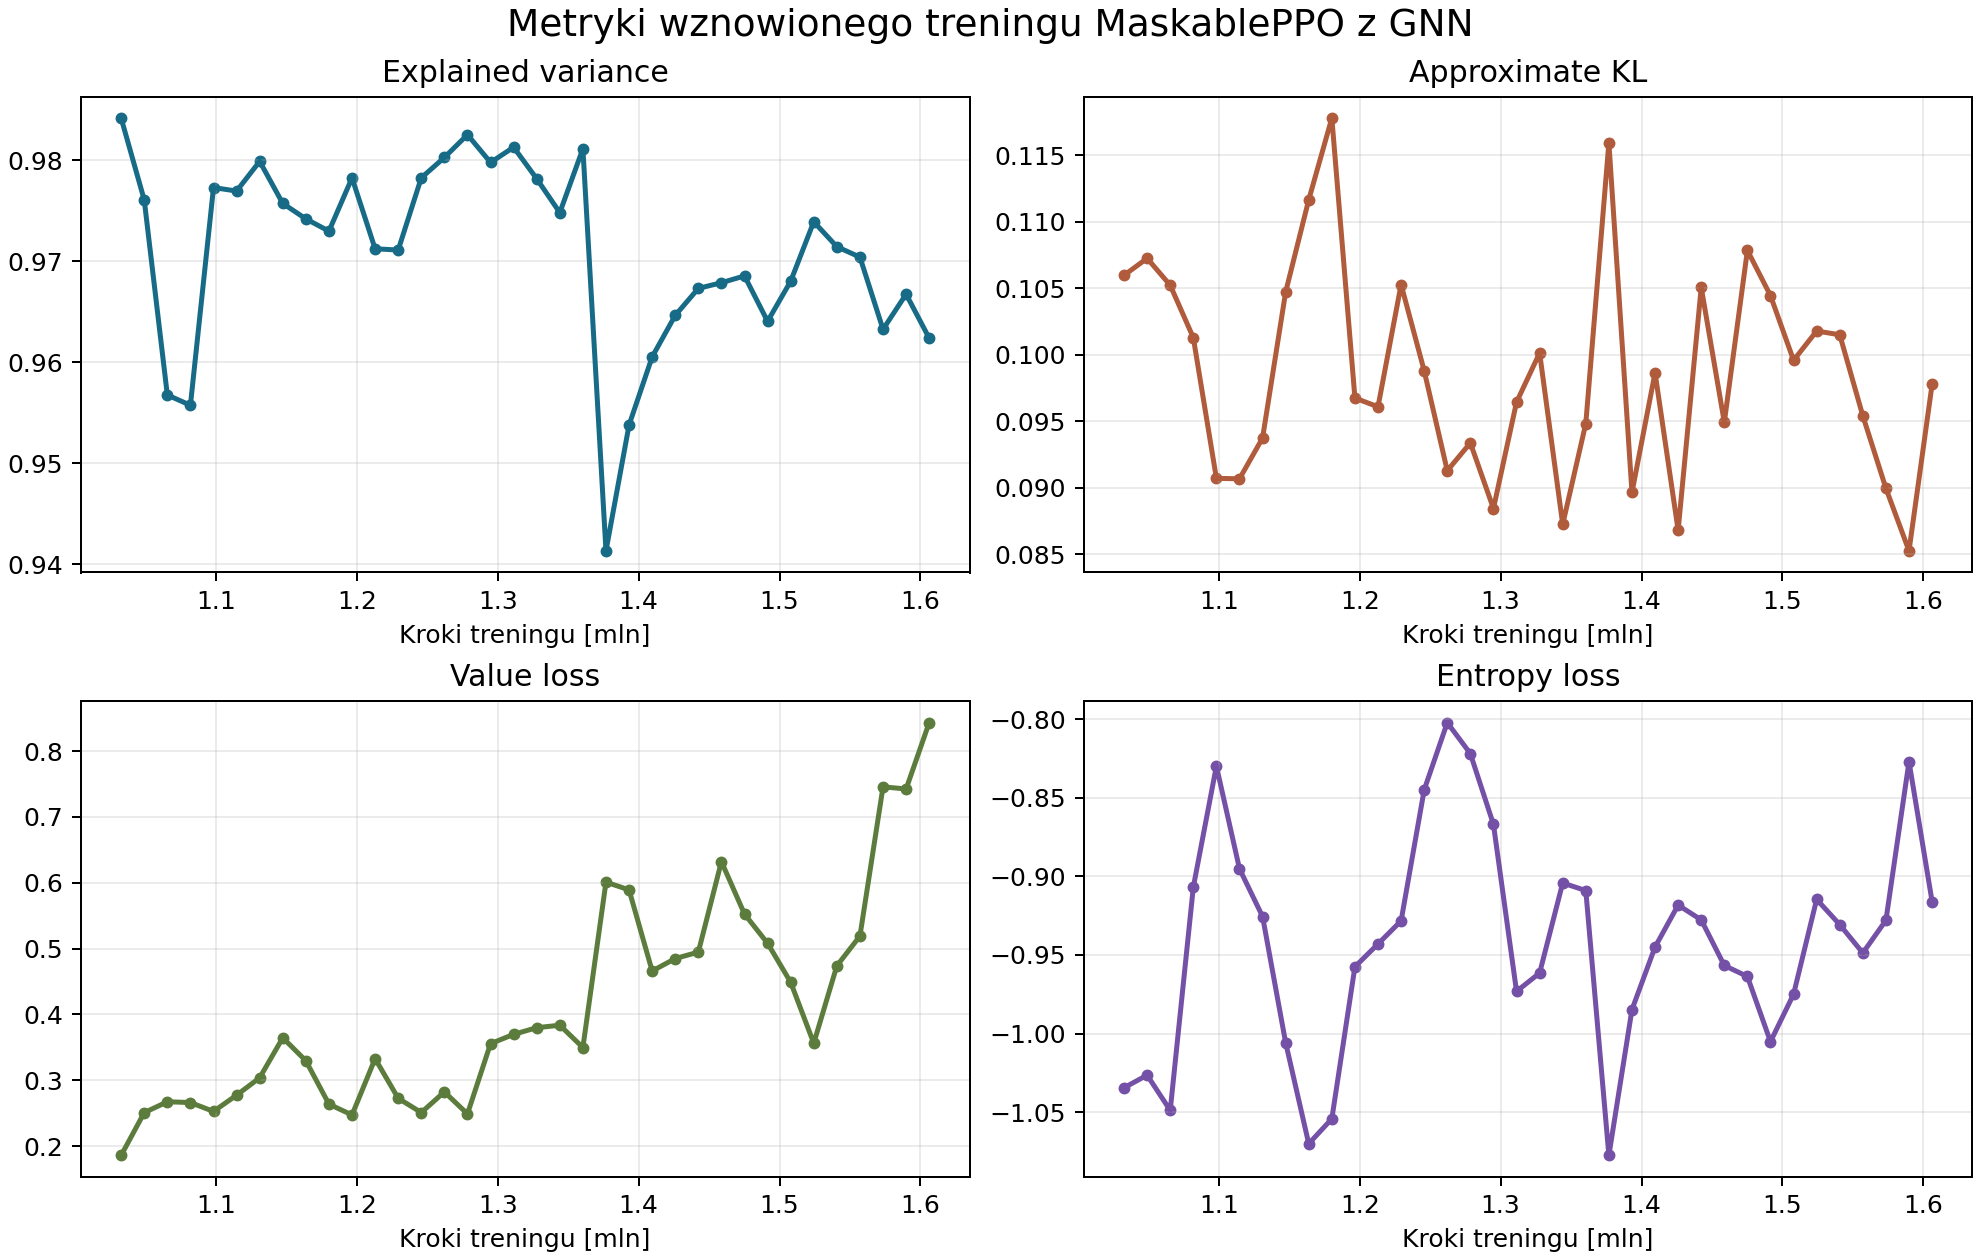
\includegraphics[width=0.94\textwidth]{training_metrics.png}
    \caption{Wybrane metryki podczas wznowionego treningu modelu GNN.}
    \label{fig:training}
\end{figure}

W końcowej części treningu explained variance utrzymywała się w przybliżeniu
między 0,96 a 0,98, co wskazuje na dobre dopasowanie krytyka do obserwowanych
zwrotów. Jednocześnie stosunkowo wysokie wartości approximate KL i clip fraction
sugerują, że aktualizacje polityki były agresywne i często podlegały
ograniczeniu PPO.

\section{Aplikacja internetowa}

Backend udostępnia endpointy:

\begin{itemize}[leftmargin=*]
    \item \code{GET /positions} i \code{GET /random\_position} --- pobieranie
    poprawnych pozycji,
    \item \code{POST /ai\_move} --- wykonanie ruchu agenta,
    \item \code{POST /move\_ranking} --- ranking do 20 legalnych ruchów.
\end{itemize}

Przed predykcją backend tworzy obserwację i maskę legalnych ruchów. Jeśli model
zwróci niepoprawną akcję lub wystąpi wyjątek, system wybiera ruch legalny jako
zabezpieczenie. Frontend umożliwia wybór pozycji, ruch przez przeciąganie lub
kliknięcie, wybór figury przy promocji, zmianę szybkości animacji, cofnięcie
pełnej tury, reset, historię w notacji SAN oraz wizualną podpowiedź.

Ranking ruchów bazuje na prawdopodobieństwach polityki. Jeżeli nie można ich
odczytać, backend stosuje różnicę heurystycznej oceny pozycji jako funkcję
zastępczą.

\section{Ewaluacja}

\subsection{Metodyka}

Model GNN z 1\,600\,000 kroków testowano przeciwko przeciwnikowi wybierającemu
losowy ruch legalny. Agent grał stroną będącą na ruchu w pozycji startowej.
Każdą partię ograniczono do 100 półruchów. Poza klasycznym wynikiem mierzono
promocje, przewagę materialną co najmniej 3 punkty i złożony sukces końcówkowy,
czyli co najmniej jedno z: wygrana, promocja lub przewaga materialna.

Plik wynikowy zawiera 61 krótkich serii po dwie partie, łącznie 122 partie.
Tak małe serie mają wysoki błąd losowy, dlatego poniżej przedstawiono również
agregację wszystkich zapisanych uruchomień.

\begin{table}[H]
\centering
\caption{Zagregowane wyniki ewaluacji przeciwko ruchom losowym.}
\begin{tabular}{lrr}
\toprule
\textbf{Metryka} & \textbf{Liczba} & \textbf{Odsetek} \\
\midrule
Wygrane & 0 & 0,0\% \\
Porażki & 2 & 1,6\% \\
Remisy lub brak rozstrzygnięcia & 120 & 98,4\% \\
Partie ucięte limitem & 104 & 85,2\% \\
Partie z promocją agenta & 108 & 88,5\% \\
Partie z przewagą materiału $\geq3$ & 33 & 27,0\% \\
Sukces końcówkowy & 108 & 88,5\% \\
\bottomrule
\end{tabular}
\end{table}

\begin{figure}[H]
    \centering
    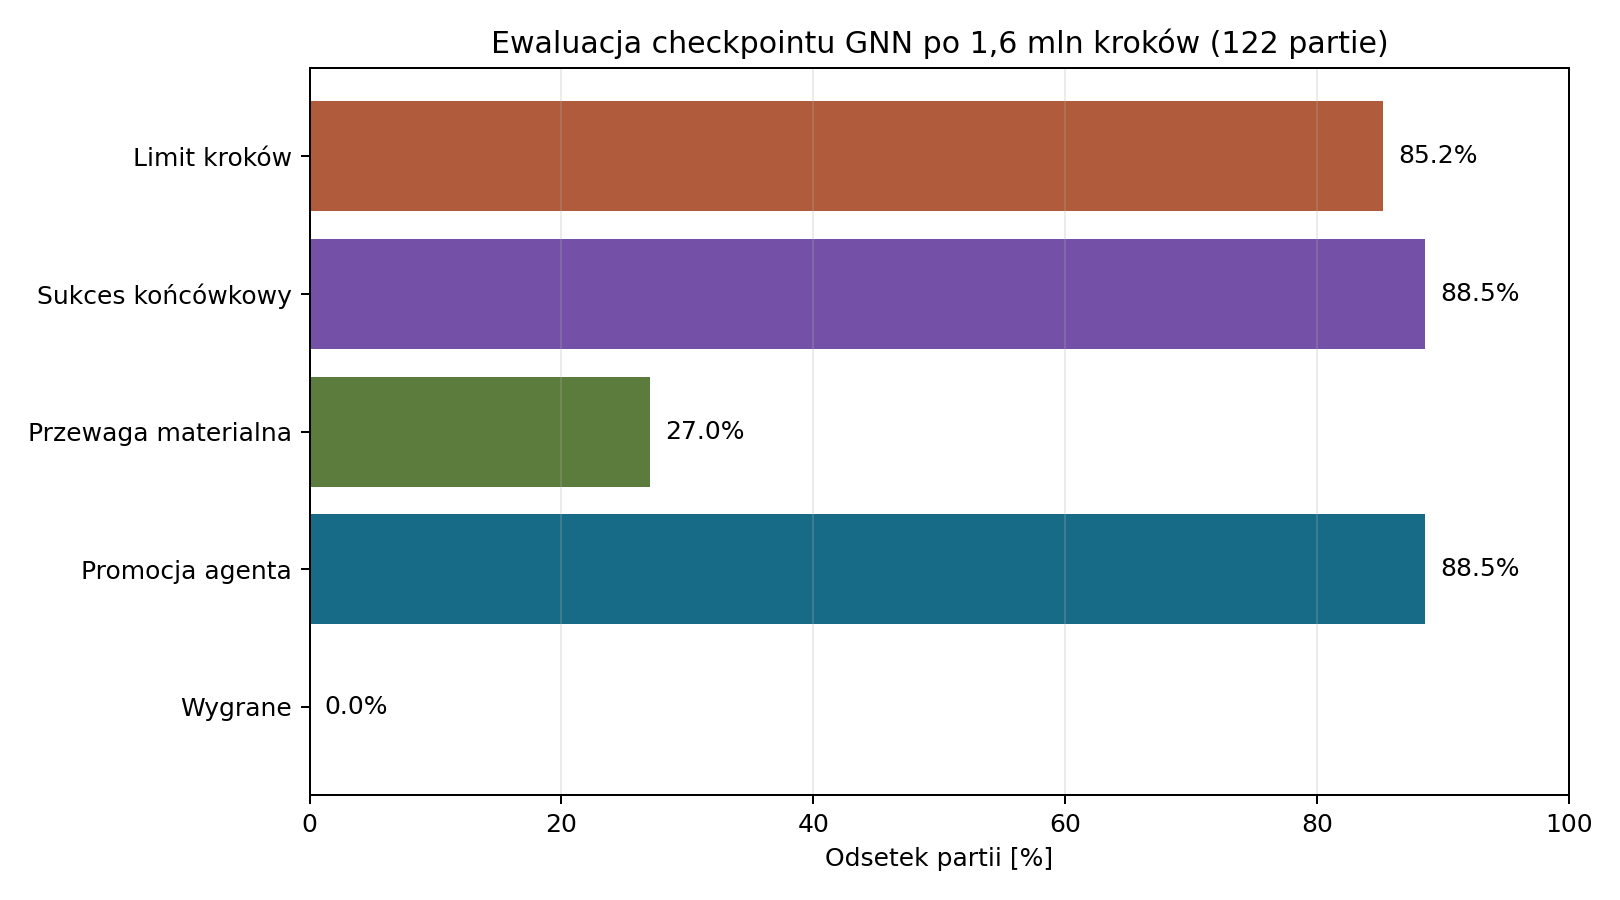
\includegraphics[width=0.82\textwidth]{evaluation_summary.png}
    \caption{Porównanie najważniejszych odsetków w ewaluacji.}
    \label{fig:evaluation}
\end{figure}

Średnia końcowa przewaga materialna wyniosła około $-0{,}62$ punktu, a średnia
nagroda około $-0{,}28$. Najbardziej widoczną umiejętnością modelu jest
doprowadzanie pionów do promocji. Brak wygranych mimo częstych promocji wskazuje,
że agent nie opanował niezawodnego matowania po uzyskaniu nowej figury albo
traci uzyskaną przewagę w długich sekwencjach.

\subsection{Ograniczenia interpretacji}

\begin{itemize}[leftmargin=*]
    \item Przeciwnik losowy jest słabym punktem odniesienia i nie pozwala ocenić
    jakości gry względem klasycznych silników.
    \item Partie ucięte limitem są liczone jako remisy, choć pozycja może być
    wygrana lub przegrana.
    \item Pozycje startowe są nieliczne, więc istnieje ryzyko przeuczenia.
    \item Ewaluacja nie używa ustalonego ziarna losowego ani jednej dużej,
    powtarzalnej próby.
    \item Plik wdrożony przez backend, \code{ppo\_chess\_model\_tuned.zip},
    używa ekstraktora spłaszczającego MLP, natomiast opisany eksperymentalny
    checkpoint 1,6 mln kroków korzysta z GNN. Przed finalnym wdrożeniem należy
    jednoznacznie wybrać i skopiować najlepszy model.
\end{itemize}

\section{Wnioski i dalszy rozwój}

Projekt realizuje pełny cykl budowy systemu inteligentnego: przygotowanie danych,
model środowiska, uczenie, zapis checkpointów, ewaluację i wdrożenie w aplikacji.
Maskowanie legalnych ruchów skutecznie dopasowuje PPO do dużej, rzadkiej
przestrzeni akcji, a ekstraktor GNN jest sensownym sposobem modelowania
geometrycznych zależności na planszy.

Najważniejszym problemem jest różnica między realizacją celów pośrednich a
formalnym zwycięstwem. Agent często promuje pionka, ale nie kończy partii.
Najbardziej wartościowe dalsze prace to:

\begin{enumerate}[leftmargin=*]
    \item rozszerzenie zbioru i rozdzielenie pozycji na zbiory treningowy oraz testowy,
    \item ocena pozycji uciętych przy użyciu Stockfisha lub tablic końcówek Syzygy,
    \item osobna nagroda za zmniejszanie dystansu do mata po promocji,
    \item trening z programem nauczania: od prostych końcówek król i pion przeciw
    królowi do struktur wielopionowych,
    \item porównanie MLP, CNN i GNN przy identycznym budżecie kroków,
    \item ewaluacja na co najmniej kilkuset partiach z ustalonymi ziarnami,
    \item wdrożenie checkpointu GNN do backendu po automatycznym teście zgodności
    wymiarów obserwacji i przestrzeni akcji.
\end{enumerate}

\section{Uruchomienie projektu}

\begin{lstlisting}[language=bash,caption={Instalacja i uruchomienie aplikacji.}]
python -m venv venv
venv\Scripts\activate
pip install -r requirements.txt

cd frontend
npm install
cd ..

uvicorn backend.main:app --reload --host 127.0.0.1 --port 8000

# w drugim terminalu
cd frontend
npm run dev
\end{lstlisting}

\begin{lstlisting}[language=bash,caption={Przykładowy trening i ewaluacja.}]
python model.py --mode train --timesteps 2000000 --n-envs 4

python eval_vs_random.py ^
  --model-path outputs/resumed_training/checkpoints/ppo_chess_gnn_checkpoint_resumed_1600000_steps.zip ^
  --games 500 ^
  --agent-color side-to-move ^
  --output outputs/eval_500.txt ^
  --csv-output outputs/eval_500.csv
\end{lstlisting}

\section*{Bibliografia}
\addcontentsline{toc}{section}{Bibliografia}

\begin{thebibliography}{9}

\bibitem{ppo}
J. Schulman, F. Wolski, P. Dhariwal, A. Radford, O. Klimov,
\textit{Proximal Policy Optimization Algorithms}, arXiv:1707.06347, 2017.

\bibitem{gae}
J. Schulman, P. Moritz, S. Levine, M. Jordan, P. Abbeel,
\textit{High-Dimensional Continuous Control Using Generalized Advantage Estimation},
arXiv:1506.02438, 2015.

\bibitem{gnn}
T. N. Kipf, M. Welling,
\textit{Semi-Supervised Classification with Graph Convolutional Networks},
International Conference on Learning Representations, 2017.

\bibitem{sb3}
A. Raffin i in.,
\textit{Stable-Baselines3: Reliable Reinforcement Learning Implementations},
Journal of Machine Learning Research, 22(268), 2021.

\bibitem{gymnasium}
Farama Foundation,
\textit{Gymnasium Documentation},
\url{https://gymnasium.farama.org/}.

\bibitem{pythonchess}
N. Fiekas,
\textit{python-chess Documentation},
\url{https://python-chess.readthedocs.io/}.

\end{thebibliography}

\end{document}
